\documentclass[3p,times]{article}
\usepackage{amsmath, amsthm, amssymb,bm,datetime}
\usepackage{graphicx,color,subfigure}
\usepackage{hyperref}
\usepackage{epstopdf}
\usepackage{booktabs}
\usepackage{cases}
\usepackage{movie15}
%% The `ecrc' package must be called to make the CRC functionality available
\newcommand{\re}{\mathbb R}
\newcommand{\Ex}[2]{\mathcal{E}^{#2}[#1]}
\newcommand{\Tr}{\mathbf{Tr}}
\newcommand{\etal}{\textit{et al. }}

\newcommand{\eq}[1]{Eq.~(\ref{#1})}
\newcommand{\Fig}[1]{Fig.~\ref{#1}}

\renewcommand{\v}[1]{\ensuremath{\mathbf{#1}}}
\newcommand{\vo}[1]{\ensuremath{\boldsymbol{#1}}}
\newcommand{\pderiv}[2]{\frac{\partial #1}{\partial #2}}

\newcommand{\eps}{\boldsymbol{\epsilon}}
\newcommand{\Nu}{\boldsymbol{\nu}}
\newcommand{\Ps}{\boldsymbol{\Psi}}
\newcommand{\xii}{\boldsymbol{\xi}}
\newcommand{\Al}{\boldsymbol{\alpha}}
\newcommand{\x}{\mathbf{x}}
\newcommand{\s}{\mathbf{s}}
\newcommand{\C}{\mathbf{C}}
\newcommand{\uu}{\mathbf{u}}
\newcommand{\z}{\mathbf{z}}
\newcommand{\q}{\mathbf{q}}
\newcommand{\A}{\mathbf{A}}
\newcommand{\B}{\mathbf{B}}
\newcommand{\f}{\mathbf{f}}
\newcommand{\hc}{\mathbf{H}}
\newcommand{\R}{\mathbf{R}}
\newcommand{\G}{\mathbf{G}}
\newcommand{\y}{\mathbf{y}}
\newcommand{\Y}{\mathbf{Y}}
\newcommand{\teta}{\boldsymbol{\theta}}
\newcommand{\Teta}{\boldsymbol{\Theta}}
\newcommand{\pe}{\hat{\mathbf{p}}}
\newcommand{\pl}{\mathbf{p}^{(l)}}
\newcommand{\pt}{\mathbf{p}^\text{true}}

\DeclareMathOperator{\Exp}{E}
\newcommand{\V}{{\mathpzc{V}}}
\newcommand{\E}{{\mathpzc{E}}}

\newcommand{\bs}{b}
\newcommand{\bv}{\mathbf{b}}
\newcommand{\bme}{z}
\newcommand{\bvm}{\tilde{\bv}}
\newcommand{\xg}{x^G}
\newcommand{\yg}{y^G}

\newcommand{\argminx}{\arg\min_X}
\DeclareMathOperator{\diag}{diag} 

\begin{document}

\title{Temperature Dependence of $T_1$ Relaxation Time: An Inverse Problem Approach}
\author{Reza Madankan}
\date{}

\maketitle

\section*{Introduction}\label{sec:intro}
The process of Magentic Resonance Laser Induced Temperature Treatment (MRLITT) as a minimally invasive local treatment of cancerous tumors has received increasing attention in recent years. Performance of MRLITT crucially depends on parameters like tissue relaxation times, known as $T_1$ and $T_2$. One of the major challenges in MRLITT process is temperature dependence of these parameters. Hence, one needs to have an accurate approximation of changes in relaxation times as a function of tissue temperature. In thid manuscript, we study the effect of the temperature of $T_1$ relaxation time. 

\section*{Problem Statement}\label{sec:prob}
It is well established that the T1 relaxation time changes as a function of temperature \cite{rieke2008mr}. In general, it is assumed that $T_1$ relaxation time linearly changes as a function of temperature $u$:

\begin{equation}\label{T1model}
T_1(u)=T_1^{ref}\left(1+m(u-u^{ref})\right)
\end{equation}
where, $u^{ref}$ denotes the tissue temperature in normal conditions and $T_1^{ref}$ represents the corresponding value of relaxation time. Coefficient $m$ denotes the sensitivity of $T_1$ relaxation time with respect to temperature $u$ and it is usually between 0.01 and 0.02 for different tissue types. Note that due to tissue dependencies of parameters $m$ and $T_1^{ref}$, it is a reasonable assumption to consider these parameters to be uncertain.

On the other hand, a measurement data is given by the following observation model

\begin{equation}
\rho = h(u)=\frac{sin(\theta)\left(1-e^{-\frac{T_r}{T_1(u)}}\right)}{sin(\beta)\left(1-cos(\theta)e^{-\frac{T_r}{T_1(u)}}\right)}+\nu,\quad \nu \sim \mathcal{N}(0,\sigma)
\end{equation}
where, $\theta$ and $\beta$ are corresponding flip angles of the experiment and $T_r$ denotes the repetition time. Note that $\beta$ is usually considered to be a small angle and $\theta \gg  \beta$ in general. 

The key goal of this article is to find a good estimate for temperature dependencies of parameter $T_1$, given a set of data observations $\rho_k$, $k=1,2,\cdots,n$. Note that the uncertainty in $T_1$ is related to uncertain parameters $m$ and $T_1^{ref}$. Hence, the problem of $T_1$ estimation is equivalent with estimating the parameters $m$ and $T_1^{ref}$.

\section*{Parameter Estimation}\label{sec:est}
We use a minimum variance framework for estimating the parameters $T_1^{ref}$ and $m$. To do so, lets first concatenate these parameters in a parameter vector $\Theta$, i.e.

\[\Theta = [T_1^{ref},\quad m]^T\]\nonumber

Note that there exist some prior statistics,e.g. mean and covariance, for the parameter $\Theta$:
\begin{equation}\label{mean}
\hat{\Theta}\equiv\Ex{\Theta}{}=\int_{\Theta} \Theta p(\Theta)d\Theta
\end{equation}
\begin{equation}\label{covar}
\Sigma\equiv\Ex{(\Theta-\Ex{\Theta}{})(\Theta-\Ex{\Theta}{})^T}{}=\int_{\Theta} (\Theta-\Ex{\Theta}{})(\Theta-\Ex{\Theta}{})^T p(\Theta)d\Theta
\end{equation}
Now, based on the minimum variance framework, posterior statistics of $\Theta$ are given as \cite{Madankan_jcp,madankan_jgcd}:
\begin{align}
\hat{\Theta}^+&=\hat{\Theta}^- + \mathbf{K}\left(\z-\Ex{h(u)}{-}\right)\label{minvar_mean}\\
\boldsymbol{\Sigma}^+& = \boldsymbol{\Sigma}^- + \mathbf{K} \boldsymbol{\Sigma}_{hh}\mathbf{K}^T\label{minvar_var}
\end{align}
where, $\z={\rho_1,\rho_2, \cdots, \rho_n}$ is the measurement vector of $n$ observations and the gain matrix $\mathbf{K}$ is given by
\begin{equation}
\mathbf{K} = \boldsymbol{\Sigma}_{\Theta h}^T\left(\boldsymbol{\Sigma}_{hh}^-+\v{R}\right)^{-1}\label{Kgain}
\end{equation}
and $\v{R}$ represent covariance matrix of the noise signal $\nu$. The matrices $\boldsymbol{\Sigma}_{\Theta h}$ and $\boldsymbol{\Sigma}_{hh}$ are defined as:
\begin{align}
\hat{h}^-&\triangleq \Ex{h(u,\Teta)}{-}=\int_{\Theta}\underbrace{h(u,\Theta)}_{h}p(\Teta)d\Teta\label{h_k}\\
\boldsymbol{\Sigma}_{\Theta h} & \triangleq\Ex{(\Teta-\hat{\Teta})(h-\hat{h}^-)^T}{-}\label{Pzy}\\
\boldsymbol{\Sigma}_{hh}^- &\triangleq \Ex{(h-\hat{h}^-)(h-\hat{h}^-)^T}{-}\label{Pzz}
\end{align}

Note that in above equations, superscripts $+$ and $-$ are used to represent posterior and prior values of the corresponding statistics.

\section*{Numerical Simulations}\label{sec:sim}
For simulation purpose, we have considered the problem of estimating $T_1$ for a set of experimental data, resulted from MRLITT.

\begin{figure} % Temp(137,127,1:50)
\centering
\begin{tabular}{cc}
\subfigure[]{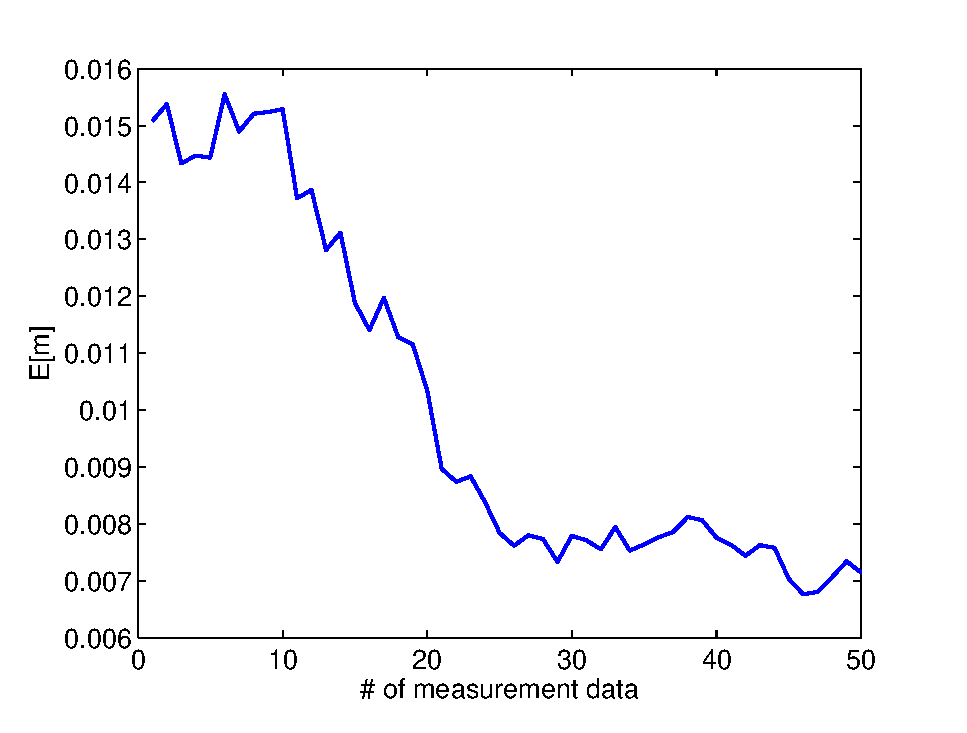
\includegraphics[width=2.5in]{mcvr.eps}} &
\subfigure[]{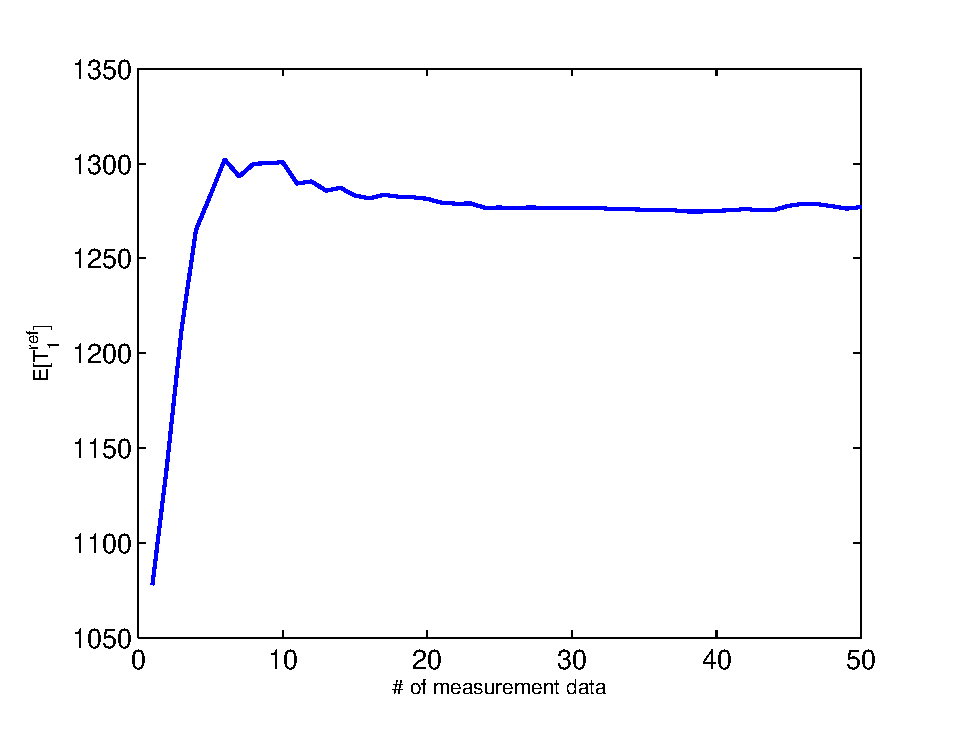
\includegraphics[width=2.5in]{T1refcvr.eps}}\\
\subfigure[]{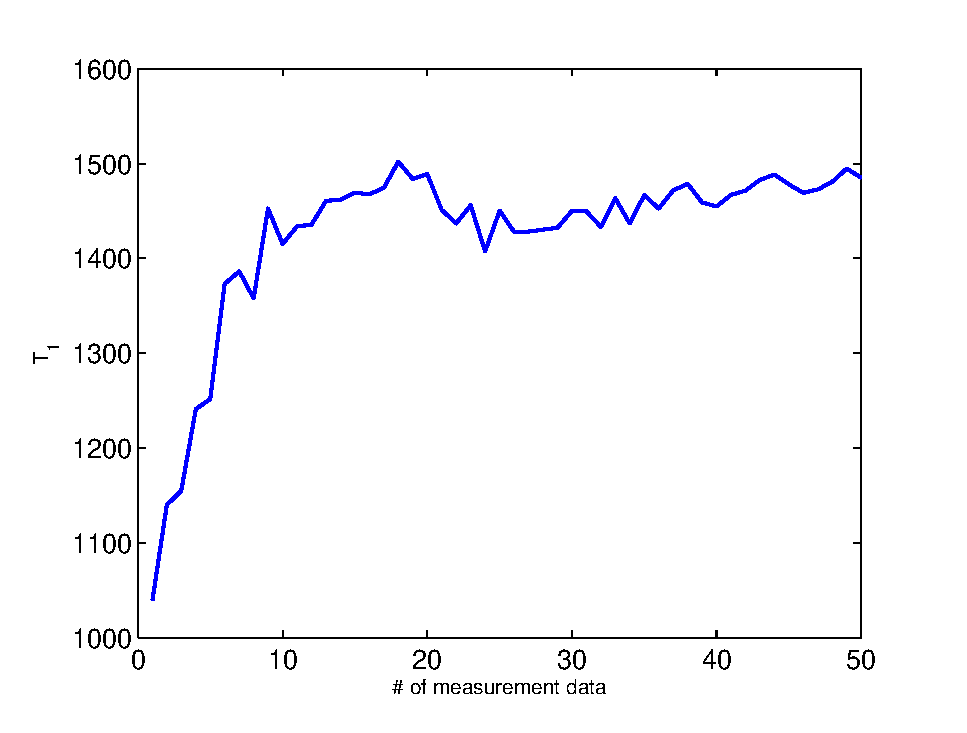
\includegraphics[width=2.5in]{T1cvr.eps}} &
\subfigure[]{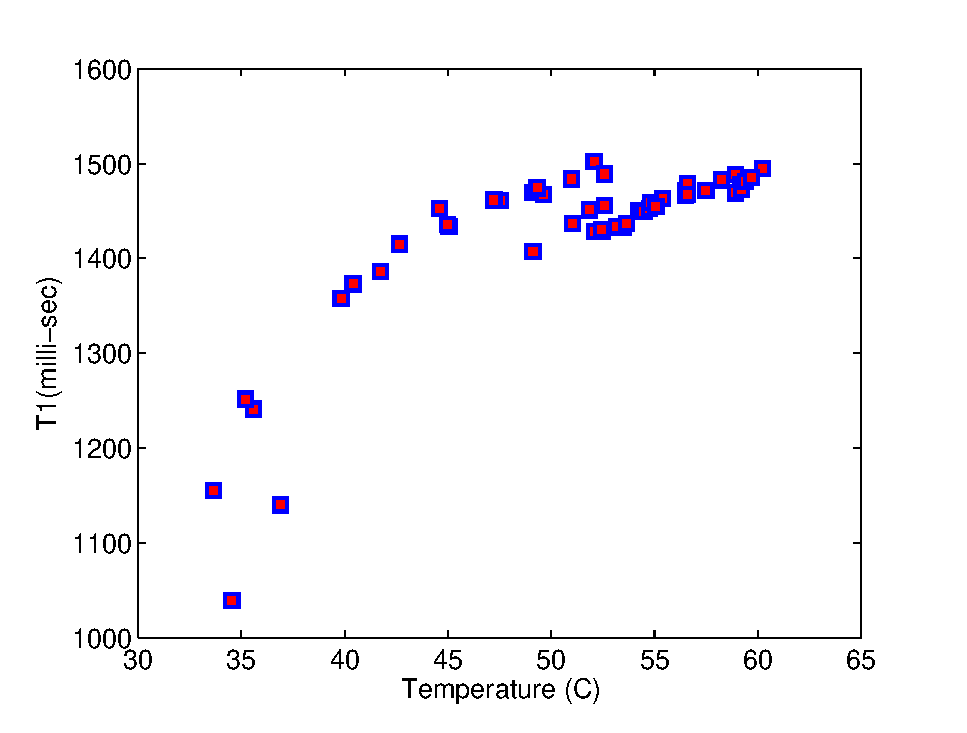
\includegraphics[width=2.5in]{T1vsTemp.eps}} 
\end{tabular}
\caption{a-c) convergence of parameter estimates versus different number of data observations a) $m$, b) $T_1^{ref}$, and c) $T_1$. Fig d) shows the variations of the estimated $T_1$ versus changes of tissue temperature.}
\end{figure}

\begin{figure}[ht]
\begin{center}
\includemovie[]{12cm}{12cm}{T1vsTemp.mp4}
\caption{Variation of $T_1$ field during the heating} 
\end{center}
\end{figure}


\begin{figure}
\centering
\begin{tabular}{cc}
\hspace{-0.6in}\subfigure[]{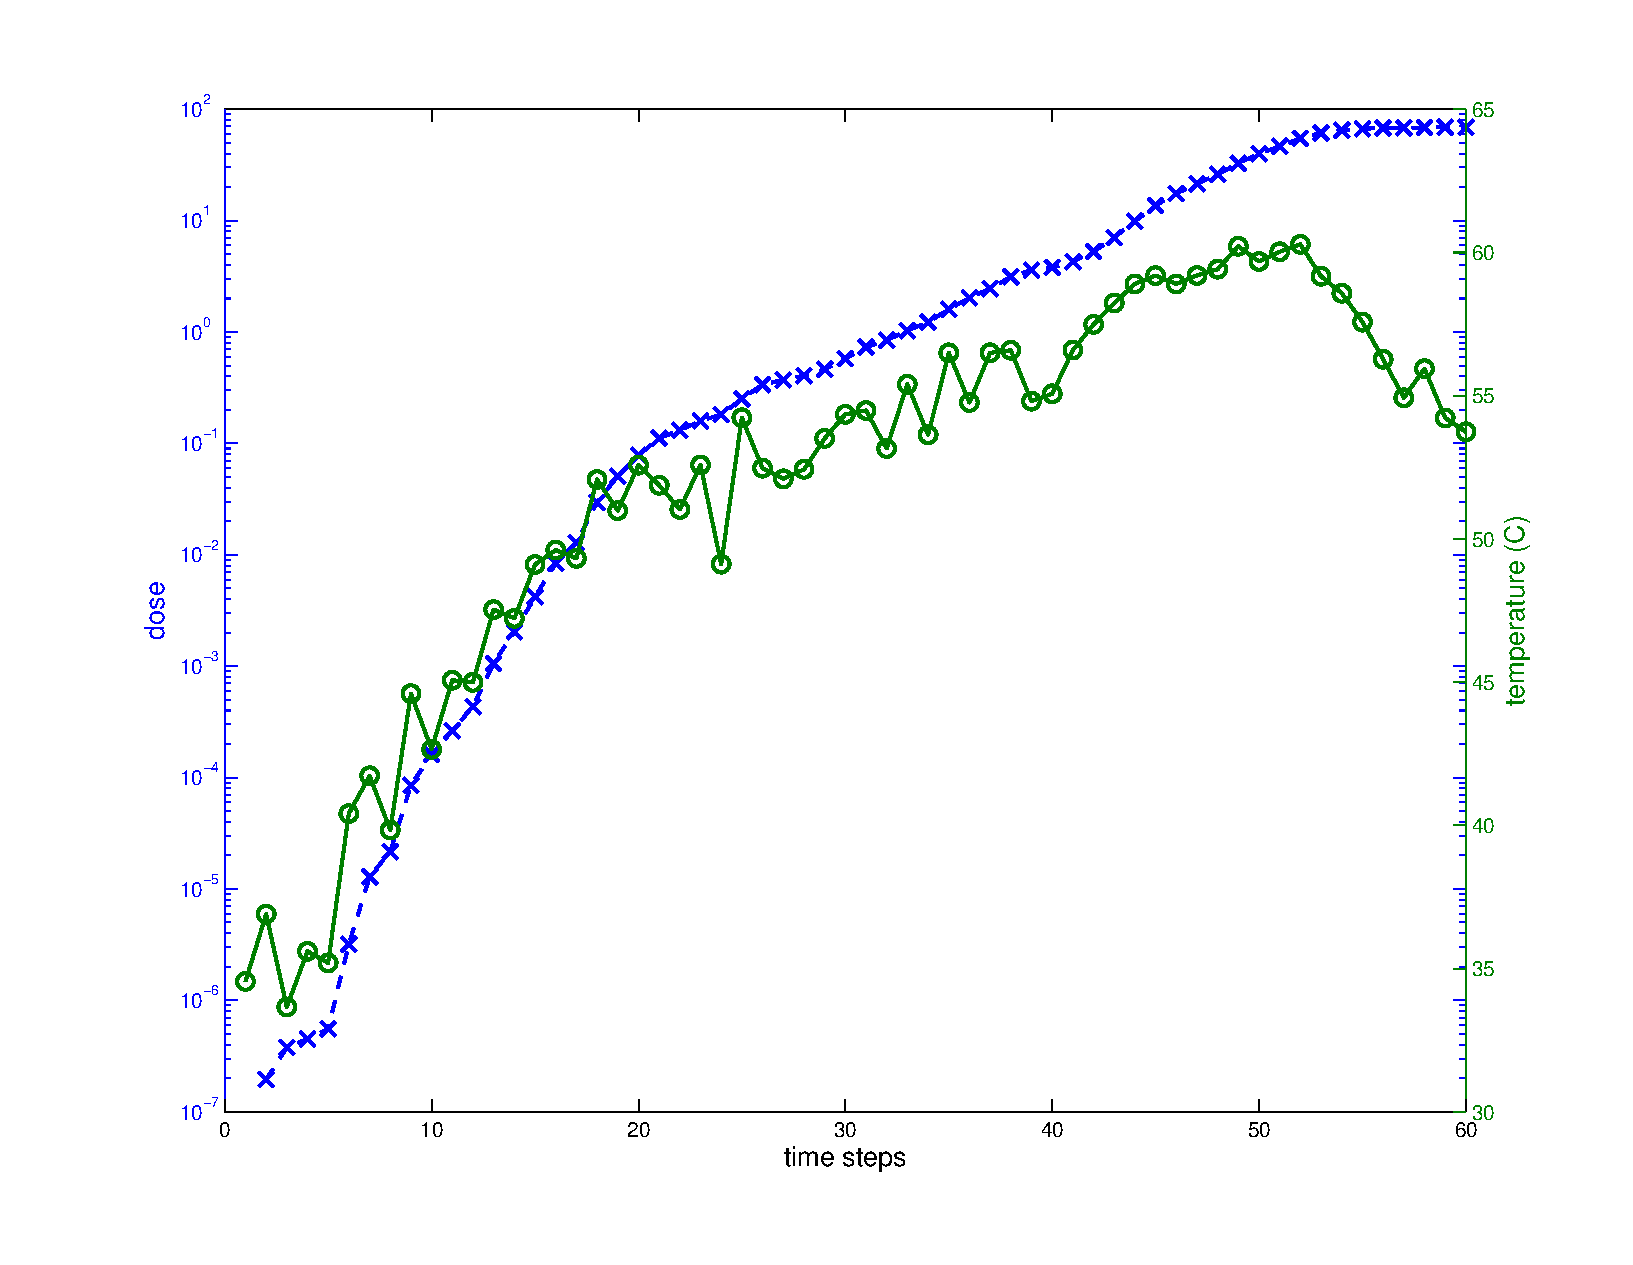
\includegraphics[width=3in]{TempDose_time.eps}} &
\subfigure[]{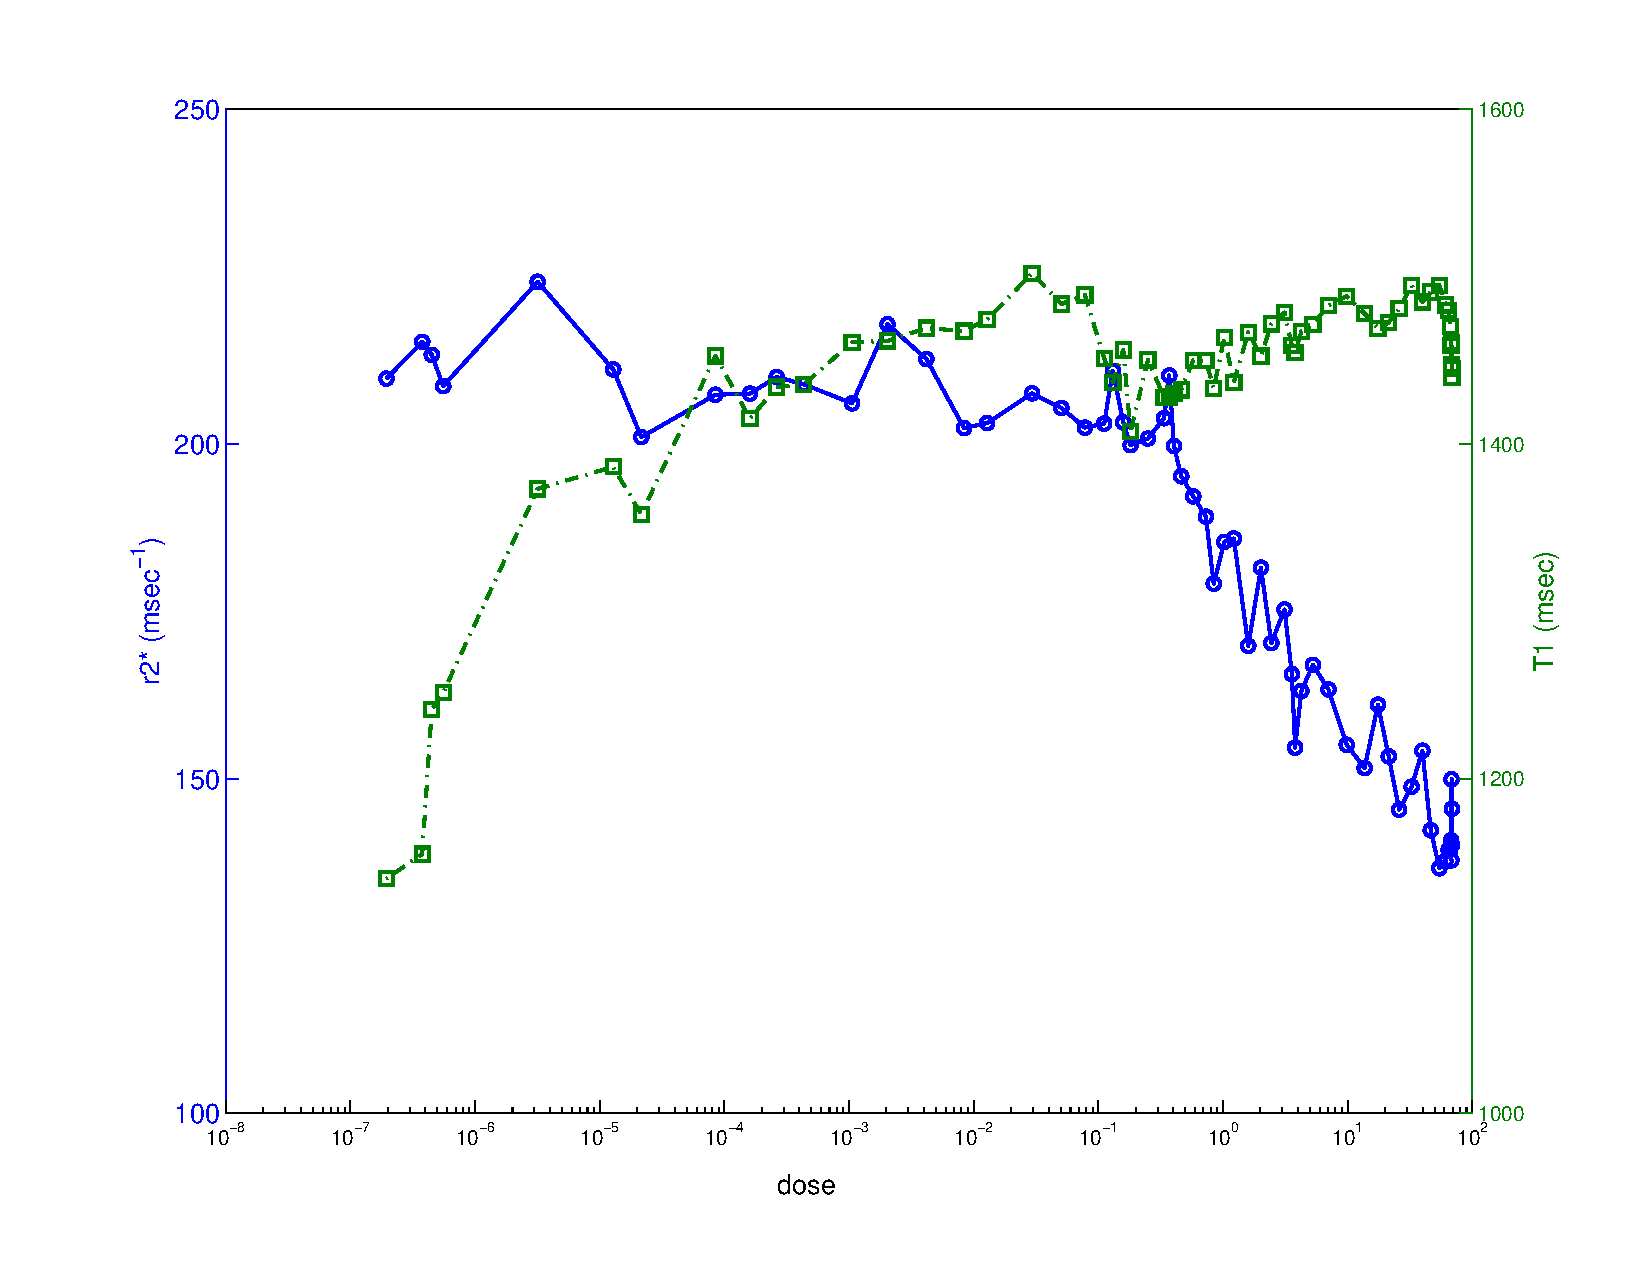
\includegraphics[width=3in]{r2starT1_dose.eps}}
\end{tabular}
\caption{a) variations of temperature and necrosis dose over time, b) variations of $r2*$ and $T1$ versus necrosis dose}\label{tempdose}
\end{figure}

\begin{figure}
\centering

{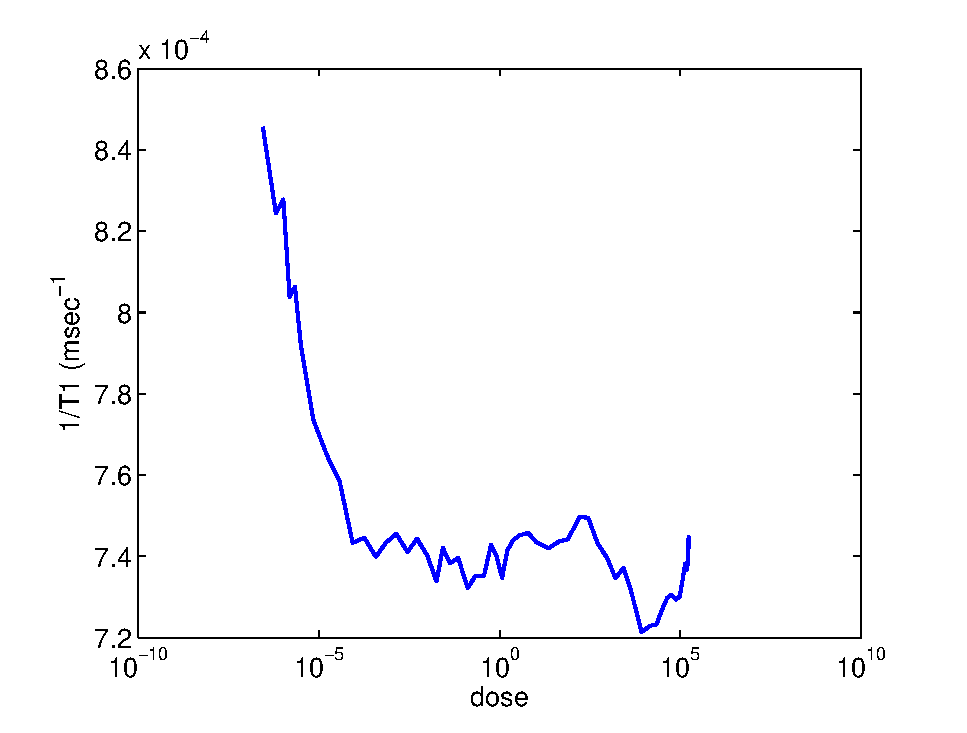
\includegraphics[width=4in]{r1_dose.eps}}
\caption{variations of $r1$ versus necrosis dose}\label{r1dose}
\end{figure}


\pagebreak
\bibliographystyle{ieeetr}
\bibliography{refs}

\end{document}